\documentclass[
  bibliography=totoc,     % Literatur im Inhaltsverzeichnis
  captions=tableheading,  % Tabellenüberschriften
  titlepage=firstiscover, % Titelseite ist Deckblatt
]{scrartcl}

% Paket float verbessern
\usepackage{scrhack}

% Warnung, falls nochmal kompiliert werden muss
\usepackage[aux]{rerunfilecheck}

% unverzichtbare Mathe-Befehle
\usepackage{amsmath}
% viele Mathe-Symbole
\usepackage{amssymb}
% Erweiterungen für amsmath
\usepackage{mathtools}

% Fonteinstellungen
\usepackage{fontspec}
% Latin Modern Fonts werden automatisch geladen
% Alternativ zum Beispiel:
%\setromanfont{Libertinus Serif}
%\setsansfont{Libertinus Sans}
%\setmonofont{Libertinus Mono}

% Wenn man andere Schriftarten gesetzt hat,
% sollte man das Seiten-Layout neu berechnen lassen
\recalctypearea{}

% deutsche Spracheinstellungen
\usepackage[ngerman]{babel}


\usepackage[
  math-style=ISO,    % ┐
  bold-style=ISO,    % │
  sans-style=italic, % │ ISO-Standard folgen
  nabla=upright,     % │
  partial=upright,   % │
  mathrm=sym,        % ┘
  warnings-off={           % ┐
    mathtools-colon,       % │ unnötige Warnungen ausschalten
    mathtools-overbracket, % │
  },                       % ┘
]{unicode-math}

% traditionelle Fonts für Mathematik
\setmathfont{Latin Modern Math}
% Alternativ zum Beispiel:
%\setmathfont{Libertinus Math}

\setmathfont{XITS Math}[range={scr, bfscr}]
\setmathfont{XITS Math}[range={cal, bfcal}, StylisticSet=1]

% Zahlen und Einheiten
\usepackage[
  locale=DE,                   % deutsche Einstellungen
  separate-uncertainty=true,   % immer Unsicherheit mit \pm
  per-mode=symbol-or-fraction, % / in inline math, fraction in display math
]{siunitx}

% chemische Formeln
\usepackage[
  version=4,
  math-greek=default, % ┐ mit unicode-math zusammenarbeiten
  text-greek=default, % ┘
]{mhchem}

% richtige Anführungszeichen
\usepackage[autostyle]{csquotes}

% schöne Brüche im Text
\usepackage{xfrac}

% Standardplatzierung für Floats einstellen
\usepackage{float}
\floatplacement{figure}{htbp}
\floatplacement{table}{htbp}

% Floats innerhalb einer Section halten
\usepackage[
  section, % Floats innerhalb der Section halten
  below,   % unterhalb der Section aber auf der selben Seite ist ok
]{placeins}

% Seite drehen für breite Tabellen: landscape Umgebung
\usepackage{pdflscape}

% Captions schöner machen.
\usepackage[
  labelfont=bf,        % Tabelle x: Abbildung y: ist jetzt fett
  font=small,          % Schrift etwas kleiner als Dokument
  width=0.9\textwidth, % maximale Breite einer Caption schmaler
]{caption}
% subfigure, subtable, subref
\usepackage{subcaption}

% Grafiken können eingebunden werden
\usepackage{graphicx}

% schöne Tabellen
\usepackage{tabularray}
\UseTblrLibrary{booktabs, siunitx}

% Verbesserungen am Schriftbild
\usepackage{microtype}

% Literaturverzeichnis
\usepackage[
  backend=biber,
]{biblatex}
% Quellendatenbank
\addbibresource{lit.bib}
\addbibresource{programme.bib}

% Hyperlinks im Dokument
\usepackage[
  german,
  unicode,        % Unicode in PDF-Attributen erlauben
  pdfusetitle,    % Titel, Autoren und Datum als PDF-Attribute
  pdfcreator={},  % ┐ PDF-Attribute säubern
  pdfproducer={}, % ┘
]{hyperref}
% erweiterte Bookmarks im PDF
\usepackage{bookmark}

% Trennung von Wörtern mit Strichen
\usepackage[shortcuts]{extdash}

\author{%
  Vincent Wirsdörfer\\%
  \href{mailto:vincent.wirsdoerfer@udo.edu}{authorA@udo.edu}%
  \and%
  Joris Daus\\%
  \href{mailto:joris.daus@udo.edu}{authorB@udo.edu}%
}
\publishers{TU Dortmund – Fakultät Physik}


\begin{document}

\section{Zielsetzung}
\label{sec:Zielsetung}

Der Franck-Hertz-Versuch ist ein grundlegendes Experiment im Hinblick auf die Diskretisierung von Energieniveaus und somit auf den quantenmechanischen 
Charakter eines Atoms. Das Experiment kann der Kategorie der \textbf{Elektronenstoßexperimente} zugeordnet werden, weshalb ein Großteil des Informationen 
aus dem Energieverlust gewonnen werden kann, welcher durch Stöße zweier Teilchen erfolgt. Ziel des Versuches ist es daher eine präzisere Vorstellung 
der Energiequantenlung innerhalb der Atomhülle zu erhalten und somit direkte Rückschlüsse auf die Energieniveaus zu ziehen.

\section{Theorie}
\label{sec:Theorie}

Wie bereits erwähnt repräsentiert der Franck-Hertz-Versuch ein Elektronenstoßexperiment. In diesem speziellen Fall lässt sich das grundlegende Prinzip 
demnach folgenderweise erklären. Die approximativ monoenergetischen Elektronen treffen auf die Atome eines Hg-Dampfes und wechselwirken dabei in Form von 
elastischen und elastischen Stößen. Hierbei besteht eine Äquivalanz zwischen jener Energie, die von den Hg-Atomen aufgenommen wird und der Energiedifferenz 
der Elektronen vor und nach dem Stoßprozess. Auf atomarer Ebene betrachtet werden die Hg-Atome von ihrem Grundzustand $E_0$ in den ersten angeregten
Zustand versetzt $E_1$. Mathematisch gilt somit der Zusammenhang 

\begin{equation*}
    E_\text{kin,vor} - E_\text{kin,nach} = E_1 - E_0
\end{equation*}, 

\noindent wobei sich die kinetische Energie des Elektrons über die Ruhemasse $m_0$ und die Geschwindigkeiten $v_\text{vor}$ vor dem Stoß bzw. $v_\text{nach}$
nach dem Stoß berechnen lässt. Um die Ermitlung der Elektronengeschwindigkeiten nachvollziehen zu können, ist es unabdingbar den allgemeinen Aufbau und die 
Funktionsweise des Franck-Hertz-Versuchs vorwegzunehmen.\\

\noindent Das Kernelement des Versuchs ist ein evakuiertes Gefäß mit Quecksilber-Dampf, welcher sich durch Sprühen winziger Tropfen langfristig einstellt.
Die Dichte das Dampfes kann dabei über die Umgebungsemperatur $T$ kontrolliert werden. Zusätzlich wird dem Gefäß ein Metalldraht aus Wolfram hinzugefügt, welcher 
durch den Anschluss einer Spannungsquelle erhitzt werden kann. Infolge des \emph{glühelektrischen Effekts} werden Elektronen emittiert und sind lokal 
um den Draht verteilt. Mittels einer positiv geladenen Elektrode können die Elektronen nun in z-Richtung beschleunigt werden. Visualisiert wird diese 
Konstruktion mithilfe der folgenden Abbildung.

\begin{figure}[H]
    \centering
    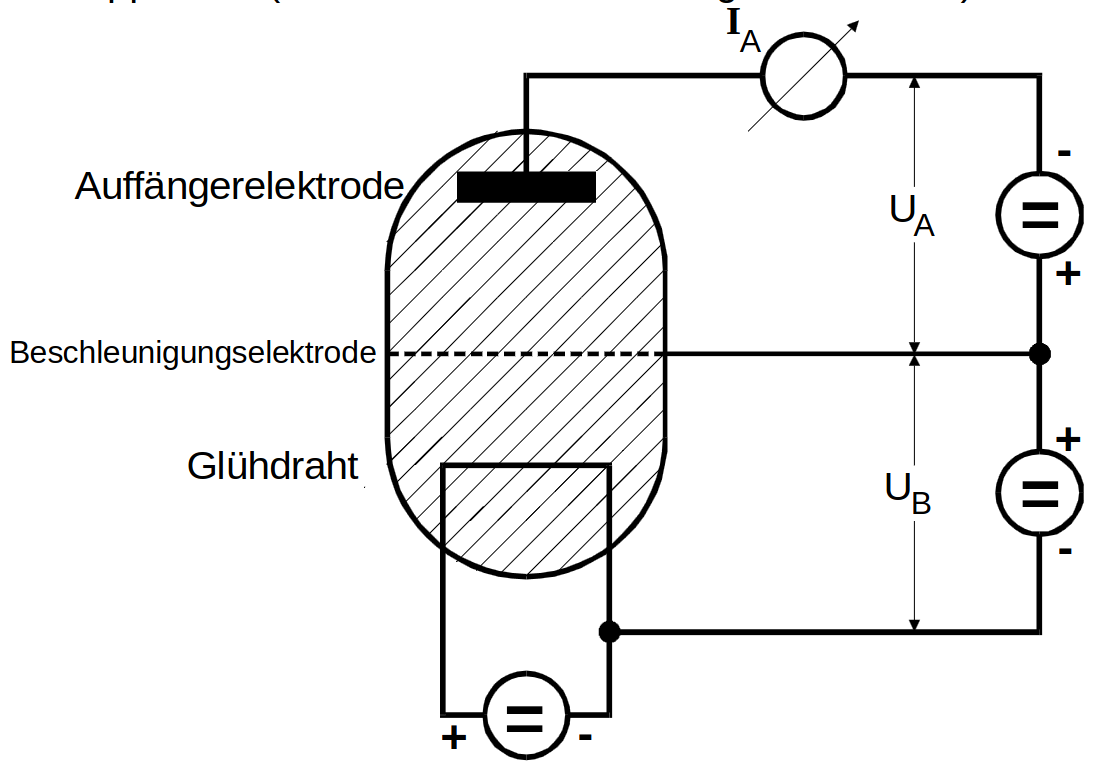
\includegraphics[height=6cm]{FH_Skizze.png}
    \caption{Skizzierter Versuchsaufbau des Franck-Hertz-Versuchs\cite{Versuchsanleitung_v601}.}
    \label{fig:FH_Skizze}
\end{figure}

\noindent Die dazu notwenige Beschleunigungsspannung wird im Folgendne als $U_\text{B}$ gekennzeichent und erfüllt die folgende Energiebilanz

\begin{equation*}
    \frac{1}{2}m_0v²_\text{vor} = e_0U_\text{B},
\end{equation*}

\noindent wobei $e_0$ die Elementarladung darstellt. Nachdem die Elektronen die Beschleunigungselektrode passieren, werden sie abgebremst. Diese ist, wie 
in Abb. \ref{fig:FH_Skizze} zu erkennen, auf die Existenz einer negativ geladenen \emph{Auffängerelektrode} zurückzuführen. Die auf der Oberfläche der
Auffängerelektrode ankommenden Elektronen bewirken einen Auffängerstrom $I_\text{A}$, welcher über ein Messinstrument ermittelt wird. Demnach werden nur 
jene Elektronen detektiert, dessen kinetische Energie größer oder gleich der von der Gegenspannung $U_\text{A}$ erzeugten elektrischen Energie ist:

\begin{equation*}
    \frac{1}{2}m_0v²_\text{z} \geq e_0U_\text{A}
\end{equation*}

\noindent Der physikalisch interaktive Bereich des Versuchs ist der Beschleunigungsraum. Hier können Elektonen und Hg-Atome miteinander wechselwirken.
Einserseits können die beiden Partner einen elastischen Stoß ausführen. Bei genauerer Betrachtung der Stoßpartner wird jedoch deutlich, warum diese Art von 
Stößen in der Bedeutung des Experiments nur eine untergeordnete Rolle spielt. Das Massenverhältnis zwischen Elektron und Hg-Atom beträgt in etwa 
$\sfrac{m_0}{M} \approx \sfrac{1}{1836}$, weshalb die Energieabgabe des Elektrons vernachlässigbar ist. Bei größer werdender Beschleunigungsspannung besitzen 
die Elektronen ausreichend kinetische Energie, um die Hg-Atome vom Grundzustand $E_0$ in den Zustand erster Anregung $E_1$ zu versetzen. Das Elektron übergibt 
somit exakt den dafür notwenigen Energiebetrag an die Hg-Atome und verbleibt ggf. mit einer Energie von $E - \left(E_1 - E_0\right)$. Nach einer gewissen
Zeit kehrt das Hg-Atom erneut in den Grundzustand zurück und emittiert dabei ein Photon der Energie 

\begin{equation*}
    E = hf = E_1 - E_2. 
\end{equation*}

\noindent Dabei steht $h$ für das Plancksche Wirkungsquantum und $f$ für die Frequenz des Lichts.\\

\subsection{Modellvorstellung der Franck-Hertz-Kurve}
\label{sec:Modellvorstellung}

\noindent Um nun einen akkuraten Überblick der Interaktionen zwischen Elektronen und Quecksilber-Atomen zu erhalten, wird der Auffängerstrom $I_\text{A}$
in Abhängigkeit der Beschleunigungsspannung $U_\text{B}$ gemessen. Idealisiert sollte dabei die folgenden Kurve zu beobachten sein:

\begin{figure}
    \centering
    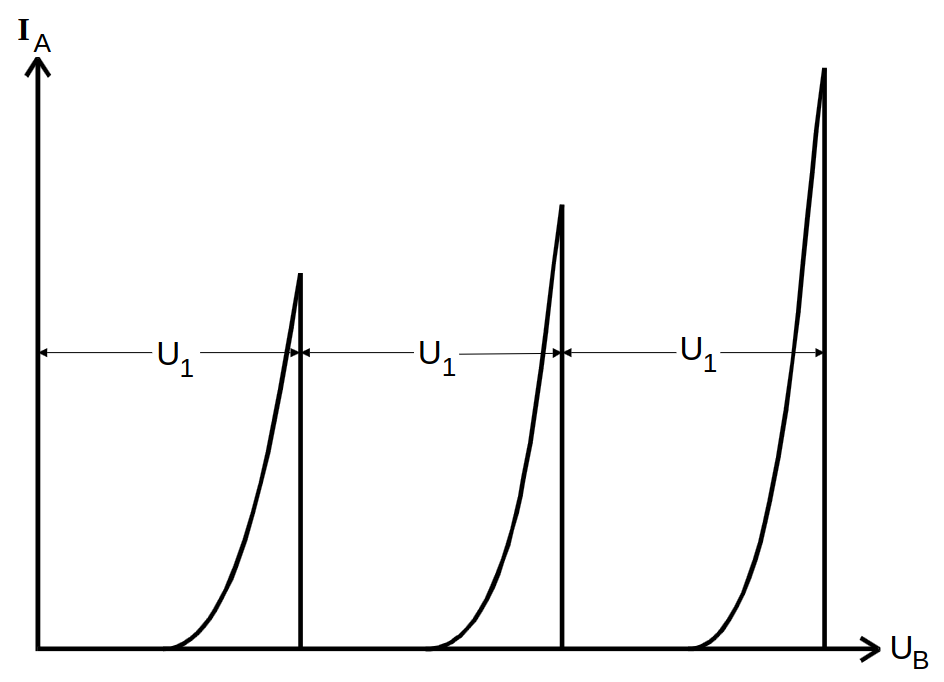
\includegraphics[height=5.5cm]{FH_Modellkurve.png}
    \caption{Modellierter Kurververlauf des Auffängerstroms als Funktion der Beschleunigungsspannung\cite{Versuchsanleitung_v601}.}
    \label{fig:FH_Modellkurve}
\end{figure}

\noindent Der erste Bereich starken Anstiegs kann auf eine leichte Erhöhung der Beschleunigungsspannung zurückgeführt werden. Die kinetische Energie der 
Elektronen reicht maximal zu elastischen Stößen mit den Hg-Atomen, was den energetischen Verlauf der Elektronen nicht wesentlich beeinflusst. Dementsprechend 
können Großteile der Raumladungswolke an die Oberfläche der Auffängerkathode gelangen, was den Auffängerstrom rasant steigen lässt. Der darauffolgende,
instantane Abfall von $I_\text{A}$ begründet sich durch unelastische Stöße unmittelabar vor der Beschleunigungskathode. Nach Abgabe der Energie $E_1 - E_0$
haben die Elektronen keine Zeit neue Energie aufzunehmen und erreichen deshalb die Auffängerkathode nicht. In dieser Modellvorstellung haben alle Elektronen 
von Beginn an die gleiche Energie, was zu einem kollektiven Abfall auf $I_\text{A} = \qty{0}{\ampere}$ führt. Bei sukzessiver Erhöhung verschiebt sich effektiv 
die Stoßzone weiter vor die Beschleunigungselektrode, sodass die Elektronen nach dem Stoß erneut genügend Energie aufnehmen können um einen Auffängerstrom 
zu erzeugen. Dieser Trend setzt sich so lang fort bis die Elektronen nach dem ersten Stoß so viel Energie aufnehmen können, um ein zweites mal zu wechselwirken.
Die zweite Stoßgrenze liegt nun unmittelbar vor der Beschleunigungselektrode, weshalb ein erneuter, unstetiger Abfall in der Kurve zu betrachten ist. Dieser 
Prozess setzt sich periodisch fort, was mithilfe der obigen Skizze verdeutlich werden soll. Der Abstand $U_1$ korrespondiert nach dieser Erklärung mit 
der ersten Anregungsenergie:

\begin{equation*}
    U_1 = \frac{1}{e_0}\left(E_1 - E_0\right)
\end{equation*}

\subsection{Realitätseinflüsse}
\label{sec:Realitaetseinfluesse}

Die im vorherigen Teilkapitel \ref{sec:Modellvorstellung} dargestellte Modellvorstellung der Franck-Hertz-Kurve entspricht nur bis zu einem gewissen Grad dem 
tatsächlichen Verlauf. Grund dafür sind Umwelteinflüsse bzw. reale Effekte, welche im Folgenen diskutiert werden.\\

\subsubsection*{Test}

tcdg




%\section{Vorbereitung}

%\section{Fehlerrechnung}
\end{document}